\subsection*{Variables definition}
\begin{itemize}
\item $i$ = user category 
\item $j$ = promotional discount: P$_0$ = 0\%, P$_1$ = 10\%, P$_2$ = 20\%, P$_3$ = 30\%
\item $p1$ = full price of the first item (\textit{Racing skis}) 
\item $p2$ = full price of second item (\textit{Racing ski helmet})
\item $p2_j$ = price of the \textit{Racing ski helmet} when applied the promo $j$
\item $c1$ = production cost of \textit{Racing skis} = 0
\item $c2$ = production cost of \textit{Racing ski helmet} = 0
\item $q1_i(p1)$ = conversion rate for user category $i$, for \textit{Racing skis} sold at the price $p1$
\item $q2_i(p2)$ = conversion rate for user category $i$, for \textit{Racing ski helmet} sold at price the $p2$
\item $s_{ji}(p2)$ = discounted price of \textit{Racing ski helmet}, for user category $i$, according to promo discount $j$
\item $d_{ij}$ = amount of promo $j$ distributed to user category $i$
\item $d_{max}$ = maximum number of promos to be to distributed (\#P$_1$ + \#P$_2$ + \#P$_3$)
\item $avgCustomer_i$ = average number of customers for category $i$
\end{itemize}


\subsection*{Formulation of elaborated variables}
\begin{itemize}
\item $p1*q1_i(p1)*avgCustomer_i$ = revenue for the sale of \textit{Racing skis} at price $p1$ to user category $i$ 
\item $s_{ji}(p2)*q2_i(s_{ji}(p2))*d_{ij}*avgCustomer_i$  = revenue for the sale of \textit{Racing ski helmet} at the discounted price $p2$, according to the promo-category assignement (note that the dependence of the second item with the first is not taken into account in this formula)
\item $(p1*q1_i(p1)-c1*q1_i(p1))*avgCustomer_i$ = revenue for the sale of \textit{Racing skis} taking into account the production cost $c1$
\item $(q2_i(p2)*(s_{ji}(p2)*q2_i(s_{ji}(p2))*d_{ij}-q2_i(s_{ji}(p2)))*c2)*avgCustomer_i$ = revenue for the sale of \textit{Racing ski helmet} taking into account the production cost $c2$
\end{itemize}

\subsection*{Objective Function}
We have a maximization problem with the following objective function:\\
\\
$\textrm {max} ( \sum \limits _{i = 0, j = 0} ^{i = 4, j = 4}[(p1*q1_i(p1) - c1*q1_i(p1) + q2_i(p2)(s_{ji}(p2)*q2_i(s_{ji}(p2))*d_{ij} -  q2_i(s_{ji}(p2))*c2))*avgCustomer_i])$

\textbf{s.t:} $ \forall j>0 : [\sum \limits _{i = 0} ^{i = 4} d_{ij}] = d_{max} $
\\
We have fixed the full prices of the two items: $p1$, $p2$. We retrieve the discounted prices of $p2$, applying the promos $j$. \\
We know: the average number of customers per category $i$, $avgCustomer_i$, the conversion rate for both products ($q1_i(p1)$, $q2_i(p2)$) and the maximum number of promos to distribute ($d_{max}$).\\
As assumption the production costs of the two items is zero ($c1$ = 0, $c2$ = 0).\\
It is possible to retrieve the total revenue for \textit{Racing skis} as the product between the full price of the first item, the conversion rate for the considered user category and the average number of customers for that category:
$(p1 * q1_i(p1) * avgCustomer_i)$.\\
For the second item the calculation of the reward is the same except for the fact that the product is buyed only if also the first one is purchased (so we multiply also the conversion rate of the first item) and the considered price have to be discounted according to the assigned promotion. 

The solution of our optimization problem consists in the distribution of the fraction of promo codes among the user categories.

\subsection*{Offline problem - designed algorithm}

We have to find the optimal solution in an offline manner (solve the maximization problem when all the parameters are known), considering the constraint that the shop uses a randomized approach to assure that a fraction of a given customer category gets a specified promotion, according to the optimal solution.\\ 
We have used an iterative approach to reach the optimal solution: we build a customer category-promotion (matching) matrix, which contains the mean expected rewards for every matching, calculated as the product between the conversion rate of the \textit{Racing ski helmet} and its discounted price.
The goal is to obtain, for each customer-promo matching, the fraction of customers that will receive this discount, in order to maximize the total reward.\\
We select the best reward for every class, for four times, retrieving, at each iteration, the four best combination of category-promotion and assigning an infinite weight to the obtained sub-optimal matching.\\
Every matching is represented by a reward configuration that maximize the total reward, every iteration is weighted and represent a different goodnesses of the solution (the first is the best, the last is the worst).\\
Through the sub-optimal matchings, we have retrieved the fractions of different promos to assign to every customer categories, based on the proportional weight of the previous sub-optimal matching. Then the retrieved proportions, are normalized category per category.

\subparagraph*{Pseudocode}
Below we schematize the previous described algorithm:\\
\begin{enumerate}
	\item For both the items fix a prices called $item1PriceFull$ and $item2PriceFull$
	\item Calculate the fraction of the customers per class that buy the first item through the conversion rate of the first item (at the predetermined price), as fractions of buyers: $firstItemBuyers[i]=$\\
	$int (customerDaily[i] * conversionRateFirstElement(item1PriceFull, i))$\\
	Once we know the number of customers that bought the first item, we aims to maximize the profit making them buy the second item.
	\item Calculate the discounted price for the different promo codes: $discountedPrice = [item2PriceFull, item2PriceFull*(1-ctx.discountPromos[1]),	item2PriceFull*(1-ctx.discountPromos[2]),item2PriceFull*(1-ctx.discountPromos[3])]$
	\item Initialize the matching matrix where the rows are the user categories and the columns are the promotions. Cells are weighted as $(conversionRateSecondItem * discountedPriceSecondItem * firstItemBuyers)$ of that class.
	\item The matching is using a Linear Sum Assignement algorithm and iterated four times, retrieving a matrix called iteration matrix. Every iteration determine the optimal solution of the matching problem which allow to maximize the profit, discarding the solution obtained in the iterations before. The iteration matrix saves all these optimal solutions.\\
	\begin{lstlisting}[basicstyle=\tiny\tt, tabsize=2, language=Python]
	for i in range(4):
		rowInd,colInd = linearSumAssignment(matchingMatrix,maximize=True)
		temp = np.zeros((4,4))
		for ind in range(0,len(rowInd)):
			temp[rowInd[ind],colInd[ind]] = matchingMatrix[rowInd[ind],colInd[ind]]
		  	  \matchingMatrix[rowInd[ind],colInd[ind]] = np.iinfo(np.int64).min
		iterationMatrix.append(temp)
	\end{lstlisting}

	\item Computing the final matrix thta holds all the distributions:\\
	\begin{lstlisting}[basicstyle=\tiny\tt, tabsize=2, language=Python]
	w = 1
	for i in range(4):
		iterSum = np.sum(iterationMatrix[i])
		coordinates = np.nonzero(iterationMatrix[i])
		for idx in range(len(coordinates[0]))
			classFinalDistribution[coordinates[0][idx], coordinates[1][idx]] = 
			  (100 *iterationMatrix[i][coordinates[0][idx], coordinates[1][idx]] /iterSum ) * w
		w = w/2
	\end{lstlisting}

	\begin{lstlisting}[basicstyle=\tiny\tt, tabsize=2, language=Python]
	for i in range(0,4):
		sumPerClass=(np.sum(classFinalDistribution[i]))
		for j in range(0,4):
			classFinalDistribution[i,j] = (classFinalDistribution[i,j]*100/sumPerClass)/100 
	\end{lstlisting}	
\end{enumerate}
\subparagraph*{Implementation} For completeness we implemented the previously described algorithm (\textit{n1.py}) and the results of the running are the following distributions matrix of promotion-category:
\begin{center}
	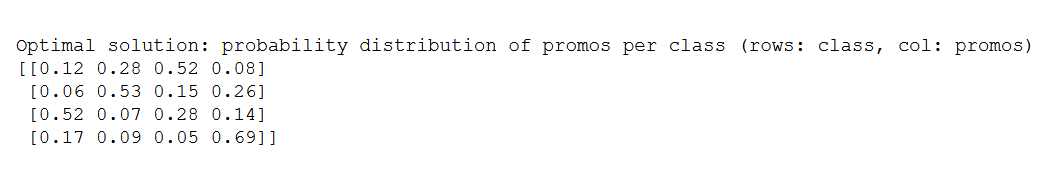
\includegraphics[scale=0.9]{Images/n1_results}
\end{center}
In terms of rewars the results are the following: 
\begin{center}
	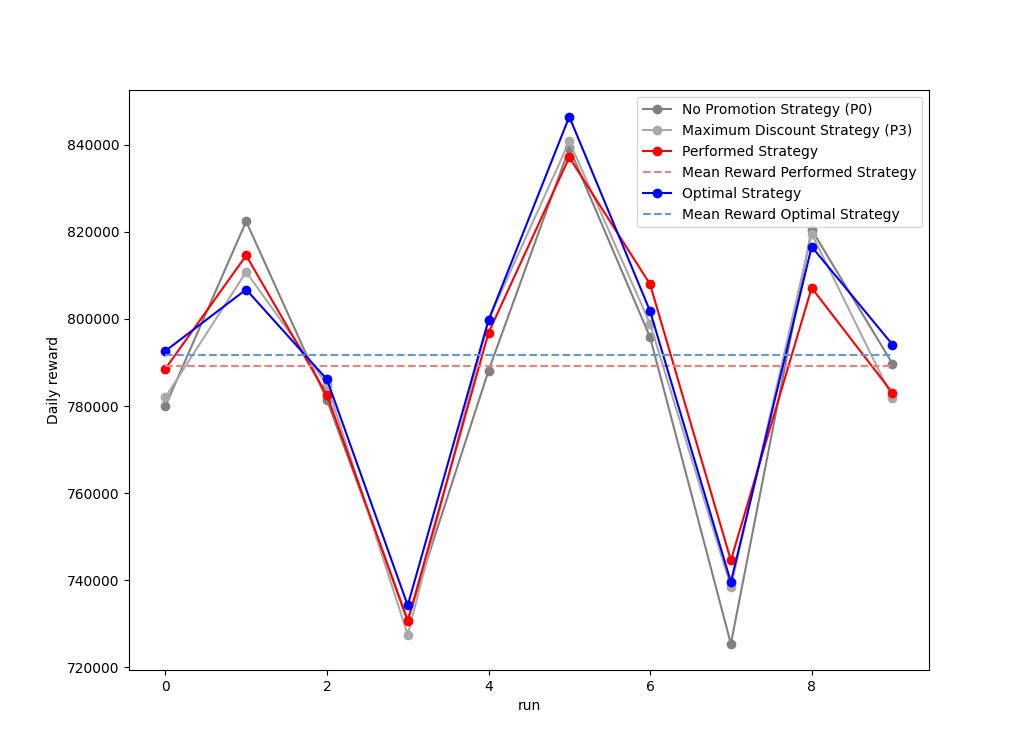
\includegraphics[scale=0.7]{Images/n1_chart}
\end{center}





